\chapter{Modely}
\label{chap:models}

% Hlavnou ulohou tejto prace je preskumat vyuzitie anotacii pri zarovnavani sekvenci... V kapitole... sme uviedli standardny parovy HMM, ktory sa na zarovnavanie sekvencii pouziva, ktory ale anotacie nevyuziva... V tejto praci sme sa to rozhodli rozdelit na dva kroky: zosumarizovat informaciu obsiahnutu v anotaciach do jedneho cisla pomocou klasifikatorov... v kapitole xxx sme navrhli dva klasifikaory, jeden pre match a druhy pre inzert, a preco su dva a nie jeden. V tejto kapitole sa venujeme tomu druhemu kroku, to znamena ako vysledok klasifikatora zaintegrovat do pHMM. ... a potom nasleduje prehlad kapitole, co v ktorej podkapitole urobime.

Hlavnou úlohou našej práce bolo preskúmať využitie dodatočnej informácie pri zarovnávaní sekvencií. Dodatočnú informáciu máme vo forme anotácií k sekvenciám. Anotácie sme sa rozhodli zakomponovať do zarovnania pomocou klasifikátorov, ktoré zosumarizujú informáciu obsiahnutú v anotáciách do jendého čísla. Prácu sme rozdelili na dve časti. Prvú časť tvorí kapitola \ref{chap:clf}, kde sme riešili problém ako základe lokálnej informácie rozhodúť, či dané pozície majú byť zarovnané k sebe alebo k medzere. Navrhli sme dva klasifikátory -- pre Match a Inzert stav, pričom prvý rozhoduje, či dané dve pozície majú byť zarovnané k sebe alebo nie. Druhý rozhoduje, či daná pozícia má byť zarovnaná k medzere.

V tejto kapitole sa venujeme druhej časti, ktorú tvorí zakomponovanie výsledkov z klasifikátorov do modelov pre zarovnávanie sekvencií. V~kapitole \ref{sec:hmm-alignment} sme si zadefinovali pHMM pre zarovnávanie sekvencií (obr. \ref{fig:simple-model}).
Najskôr si popíšeme architektúry našich dvoch modelov, ktoré sú založené na pHMM, pričom pHMM sme modifikovali tak, aby zahŕňal výstupy z klasifikátorov. Potom sa budeme venovať trénovaniu jednotlivých modelov a nakoniec si modely porovnáme a zhodnotíme ich úspešnosť.

% V~našom riešení sme predstavili 2 modifikácie pôvodného pHMM na zakomponovanie dodatočnej informácie, s využitím klasifikátorov. V~oboch modeloch sú klasifikátory rovnaké, aj s~rovnakým postupom trénovania. Líši sa len trénovanie samotného pHMM a architektúra modelu.

\section[Integrácia pHMM a klasifikátorov]{Integrácia párových HMM a výsledkov z klasifikátorov}

% Podkapitoly 4.1 a 4.2 by som zlucil do jednej (vo vseobecnosti, jednostranove pripadne odstavcove podkapitoly nie su dobry napad, to vyzera ako keby si si najskor spravil osnovu podkapitol a potom ju naplnal a do niektorych si nemal co napisat... co aj tak bolo, ale nemusime to vsetkym dat na vedomie ;)

% Takze by som dal jednu kapitolu 4.1 s nazvom "Integracia parovych HMM a vysledkov klasifikatorov".
% Tuna by som najskor porozpraval o predstave klasifikatora ako dvojrozmernej pasky (to je koniec koncov uzitocna predstava aj pri modely A), ak by sa dal urobit nejaky pekny farebny obrazok povedzme 30x30, ktory ma na farebnej skale vyznacene tie vysledky klasifikacie, tak to by bolo pekne (pripadne to urobit na nerepetitivnej sekvencii a na repetitivnej sekvencii, kde to nebude az take strukturalne jednoduche). To by mohlo tvorit uvod ku podkapitole a potom by sme mohla mat dalsie podkapitoly s nazvami:
% 4.1.1 Definicie modelov
% 4.1.2 Diskretizacia skore klasifikatorov

% V tejto kapitole si najskôr zadefinujeme dva modely -- model s klasifikátorom ako emisiou, ktorý budeme označovať model A a model s klasifikátorovou páskou, ktorý budeme označovat ako model B. Pri modeli B si uvedieme jeho dve verzie -- diskrétnu a spojitú. Porozprávame si aj o diskretizácii skóre klasifikátorov pre diskrétnu verziu modelu B.

Pri zarovnávaní sekvencií si klasifikátor z ktorého zoberieme výstup vyberieme podľa toho, v ako stave sa práve nachádzame. Pri Viterbiho algoritme konštruujeme dvojrozmernú tabuľky dynamického programovania, v ktorých sú na políčku $(i, j)$ optimálne hodnoty pre zarovnania končiace na $i$-tej pozícii v sekvencii $X$ a na $j$-tej pozícii v sekvencii $Y$. Okrem toho si pamätáme aj od kiaľ sme do daného políčka prišli. Do týchto tabuliek si môžme pridať aj informáciu o výstupe klasifikátora. To ktorý klasifikátor použijeme závisí od smeru, ktorým sme sa pohli. Ak sme sa pohli diagonálne, použijeme Match klasifikátor, ináč Indel klasifikátor.

Ak teda pridáme k zarovnaniu pásku s výstupom klasifikátora, môžme si ju predstaviť ako cestu v tabuľke, ktorá zodpovedá ceste zarovnania
(obr. \ref{fig:clf-tape}). Takúto pásku využijeme v jednom z našich modelov, ktoré definujeme v nasledujúcej sekcii.
\begin{figure}[htp]
    \centering
    \begin{subfigure}[m]{0.5\textwidth}
    \centering
    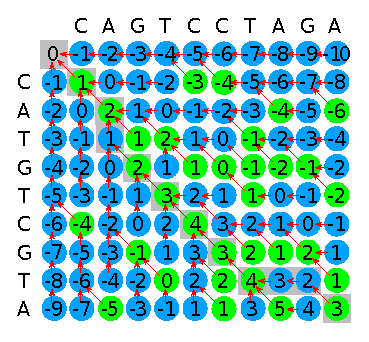
\includegraphics[width=\textwidth]{images/clf_tape}
    \end{subfigure}
    ~
    \begin{subfigure}[m]{0.3\textwidth}
    \centering
    \begin{BVerbatim}[commandchars=\\\{\}]
    CATGTCAT--A
    CA-GTCCTAGA
    {\color{green}MM}{\color{blue}I}{\color{green}MMMMM}{\color{blue}II}{\color{green}M}
    \end{BVerbatim}
    \end{subfigure}
    \caption[Použité klasifikátory v klasifikátorovej páske]{Použité klasifikátory v klasifikátorovej páske pri zarovnávaní sekvencií. Pre jednoduchosť je použitá tabuľka z algoritmu Needelman-Wunch (kapitola \ref{subsec:global-alignment}) na globálne zarovnanie sekvencií. Viterbiho algoritmus používa tri tabuľky a cesta zarovnania vedie cez všetky tri. Zelenou farbou sú označené políčka, kde sa použije Match klasifikátor, modrou sú políčka, kde sa použije Indel klasifikátor. Šedou je vyznačené zarovnanie spolu s klasifikátorovou páskou pre zarovnanie. Vpravo je vypísané to isté zarovnanie spolu s klasifikátormi z klasifikáotrovej páske.}
    \label{fig:clf-tape}
\end{figure}


\subsection{Definície modelov}

% V 4.1.1 by si navyse mohol uviest aj nejake vzorceky, tzn. ako je vlastne presne formalne zadefinovana pravdepodobnost (resp. skore pri modely A). Tiez nikde nepises, ako to ovplyvnuje dekodovacie algoritmy (resp., ze tieto modifikacie nemaju vplyv na dekodovacie algoritmy).

Prvým modelom je \textit{model s klasifikátorom ako emisiou (ďalej len model A)}. Tento model vyzerá rovnako ako základný model, aj pravdepodobnosti prechodov zostanú rovnaké, ale emisnú pravdepodobnosť nahradíme výstupom z~klasifikátora.
\begin{figure}[htp]
    \centering
    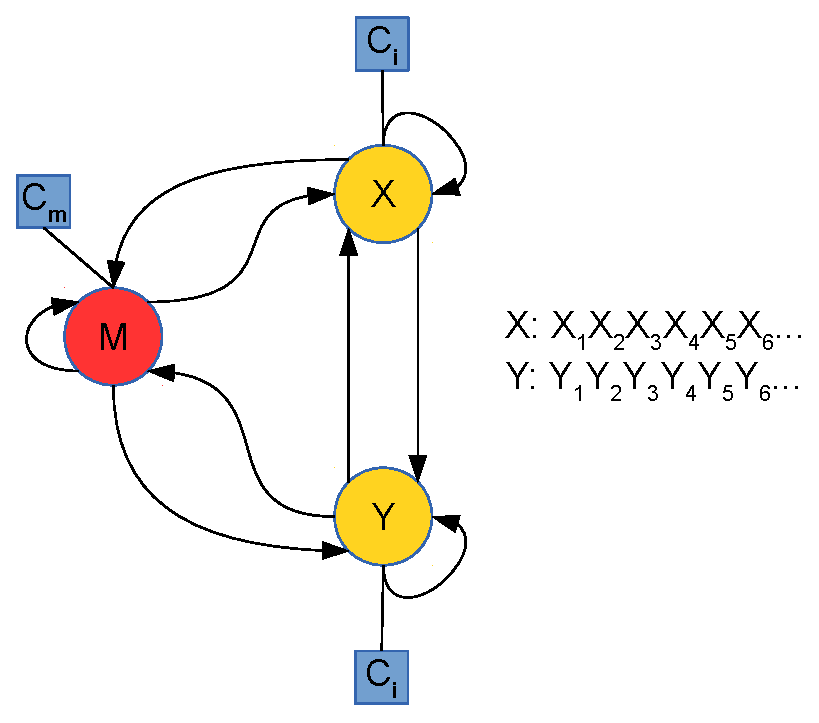
\includegraphics[width=.5\textwidth]{images/model_clf}
    \caption{Model s~klasifikátorom ako emisiou}
\end{figure}

V základnom modeli pre zarovnanie (kapitola \ref{sec:hmm-alignment}) je pravdepodobnosť emisie v match stave $P(X=x \wedge Y=y),$ kde $X, Y$ sú náhodné premenné pre bázy v sekvenciách $X$ a $Y$ a $x, y$ sú konkrétne bázy. Pre Inzert stavy analogicky.
Narozdiel od toho, výstup klasifikátora je definovaný ako $P(C=1 | W=w),$ kde $C \in \{0,1\}$ je náhodná premenná pre výstupnú triedu, pričom nula znamená, že dáta nemajú byť zarovnané k sebe a 1 znamená, že majú byť, $W$ je náhodná premenná pre okno klasifikátora, zahŕňajúce všetky atribúty a $w$ je konkrétna hodnota okna.
Pre porovnanie, ak by sme mali Match klasifikátor, a ako atribúty len príslušné bázy bolo by to $P(C=1 | X=x \wedge Y=y)$. Vidíme teda, že tieto dve pravdepodobnosti sú definované ináč a zatiaľ čo
$$\sum_{x \in X, y \in Y} P(X=x \wedge Y=y) = 1,$$
pre $\sum_{x \in X, y \in Y} P(C=1| W=w)$ takáto rovnosť neplatí.
Viterbiho algoritmus však bude fungovať aj s hodnotami $P(C=1| W=w)$ namiesto emisií a bude hľadať zarovnanie, ktoré bude maximalizovať súčin s týmito hodnotami.
O takomto modeli už však nemôžme hovoriť ako o pravdeopdobnostnom, ani ako o pHMM. Tento model je len inšpirovaný pHMM.


% Problémom tohto modelu je, že výstup klasifikátora nezodpovedá emisným pravdepodobnostiam, ale akejsi istote klasifikátora o~tom, že dve pozície majú byť zarovnané k~sebe. Hodnoty z~klasifikátora teda nesčitujú do jedna a model nie je korektný pravdepodobnostný model. V~praxi sa však ukázalo (viď sekcia \ref{sec:cmp-model}), že to až tak nevadí, avšak o~takomto modeli už nemôžeme hovoriť ako o~pravdepodobnostnom. Je len inšpirovaný pHMM.

% \section[Model s~klasifikátorovou páskou]{Model s~klasifikátorovou páskou (Model B)}
% \label{sec:model-tape}

Keďže predošlý model nie je korektný pravdepodobnostný model, navrhli sme alternatívny model, \textit{model s~klasifikátorovou páskou (ďalej len model B)}, ktorý navyše modeluje aj výstup z~klasifikátora a teda je korektný pravdepodobnostný model.
Nemodelujeme len dvojicu sekvencií, ale aj sekvenciu výstupov klasifikátora vo forme pásky, ktorú sme si definovali na začiatku kapitoly \ref{chap:models}.
Pásku s~výstupom z~klasifikátora považujeme za akúsi pomôcku pre náš zarovnávač.
\begin{figure}[htp]
    \centering
    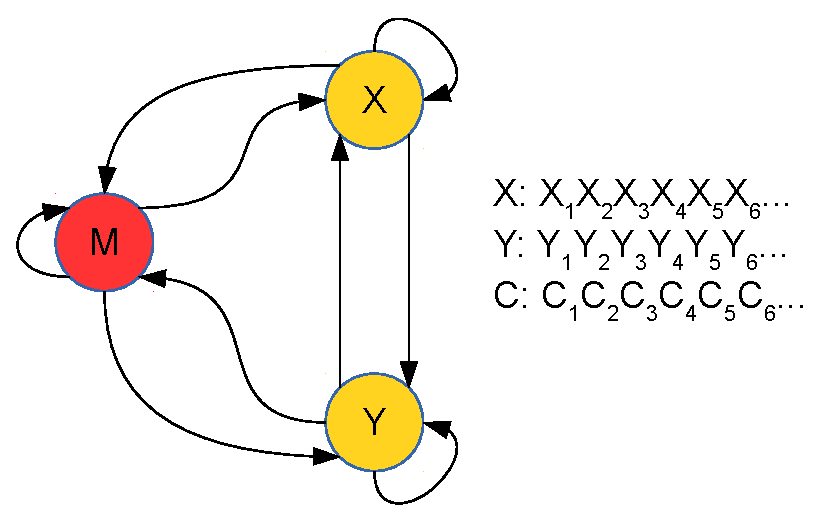
\includegraphics[width=.5\textwidth]{images/model_clf_paska}
    \caption{Model s~klasifikátorovou páskou}
\end{figure}
Klasifikátor môže vrátiť ľubovoľnú hodnotu z~intervalu $\left<0,1 \right>$. Keďže výstup z~klasifikátora je spojitý, museli sme sa s týmto problémom vysporiadať. Preto sme navrhli dve varianty tohto modelu -- diskrétnu a spojitú.

V diskrétnom modeli sme hodnoty klasifikátora rovnomerne rozdelili na $b$ hodnôt a výstup sme zaokrúhlili na najbližšiu z nich. V našich modeloch sme zvolili $b=10$.

Alternatíva k~predošlej metóde je použiť spojitý HMM. Hlavný rozdiel medzi spojitými a diskrétnymi HMM je, že spojité HMM nepočítajú s~pravdepodobnosťou, ale s~hustotou. Hodnota hustoty v~danom bode na rozdiel od pravdepodobnosti môže byť aj väčšia ako jedna. Podľa  \cite{huang1989multiple}, jedným zo štandardných spôsobov reprezentácie hustoty v~spojitých HMM je zmes gausiánov, takže využijeme interpoláciu takouto distribúciou a to budeme brať ako hustotu výstupu klasifikátora (obr. \ref{fig:clf-discretisation-2}).

% Keďže stále ide o~párový HMM, pásku si musíme predstaviť ako cestu v~2D tabuľke výstupov klasifikátorov, ktorá sa zhoduje s~cestou zarovnania. Teda ak sa pohneme horizontálne  alebo vertikálne, používame Indel klasifikátor a ak sa pohneme diagonálne tak použijeme Match klasifikátor.


\subsection{Diskrétizácia skóre klasifikátorov}

Pre diskrétnu verziu modelu B sme sa zaoberali spôsobom diskretizácie.
Diskretizovať hodnoty môžme dvoma spôsobmi. Buď jednoducho spočítame histogram pre trénovacie dáta, alebo interpolujeme vstupnú vzorku pomocou spojitej distribúcie, napr. pomocou zmesi gausiánov (tak ako v spojitej verzii) a potom toto rozdelenie diskretizujeme (obr. \ref{fig:clf-discretisation}). Druhá spomenutá metóda má výhodu v~tom, že vyhladí šum a doplní chýbajúce dáta, ale keďže je pouzitá aproximácia, zavádza určitú nepresnosť.
V~oboch prípadoch si musíme zvoliť počet košov $b$, do ktorých dáta rozdelíme. Koše sme rozdelili rovnomerne a na základe experimentov (tabuľka \ref{tab:success-b-tape}) sme si zvolili $b = 10$.

\begin{figure}[htp]
        \centering
        \begin{subfigure}[c]{0.3\textwidth}
                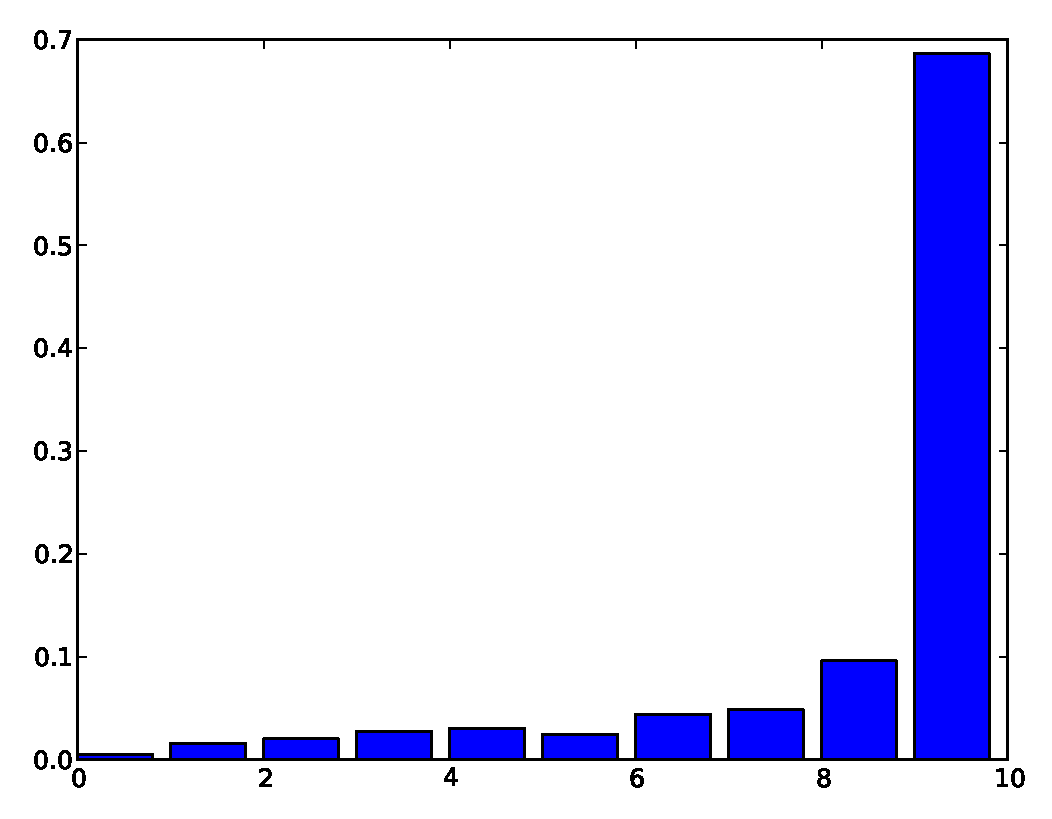
\includegraphics[width=\textwidth]{images/hist1}
                \caption{Histogram}
                \label{fig:clf-discretisation-1}
        \end{subfigure}%
        % \qquad\qquad %add desired spacing between images, e. g. ~, \quad, \qquad etc.
          %(or a blank line to force the subfigure onto a new line)
          % $\Rightarrow$
        $\vcenter{\hbox{\raisebox{.8cm}{\Huge\pointer}}}$
        \begin{subfigure}[c]{0.3\textwidth}
                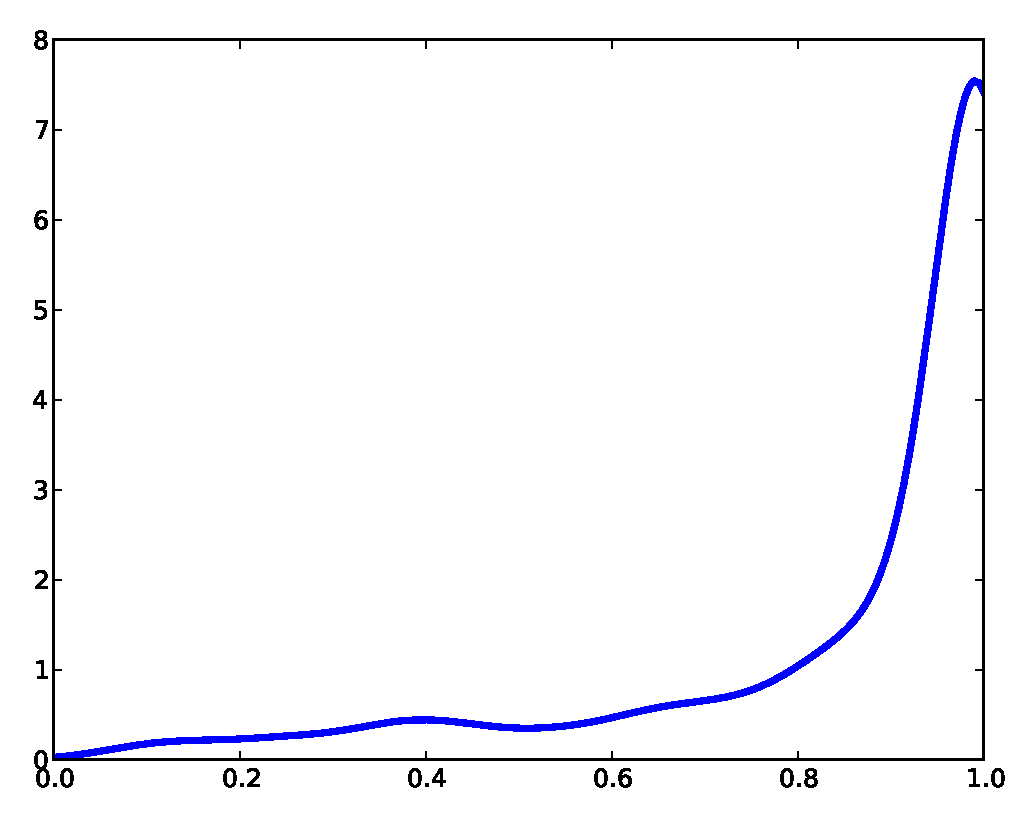
\includegraphics[width=\textwidth]{images/hist2}
                \caption{Zmes gausiánov}
                \label{fig:clf-discretisation-2}
        \end{subfigure}
        $\vcenter{\hbox{\raisebox{.8cm}{\Huge\pointer}}}$
        \begin{subfigure}[c]{0.3\textwidth}
                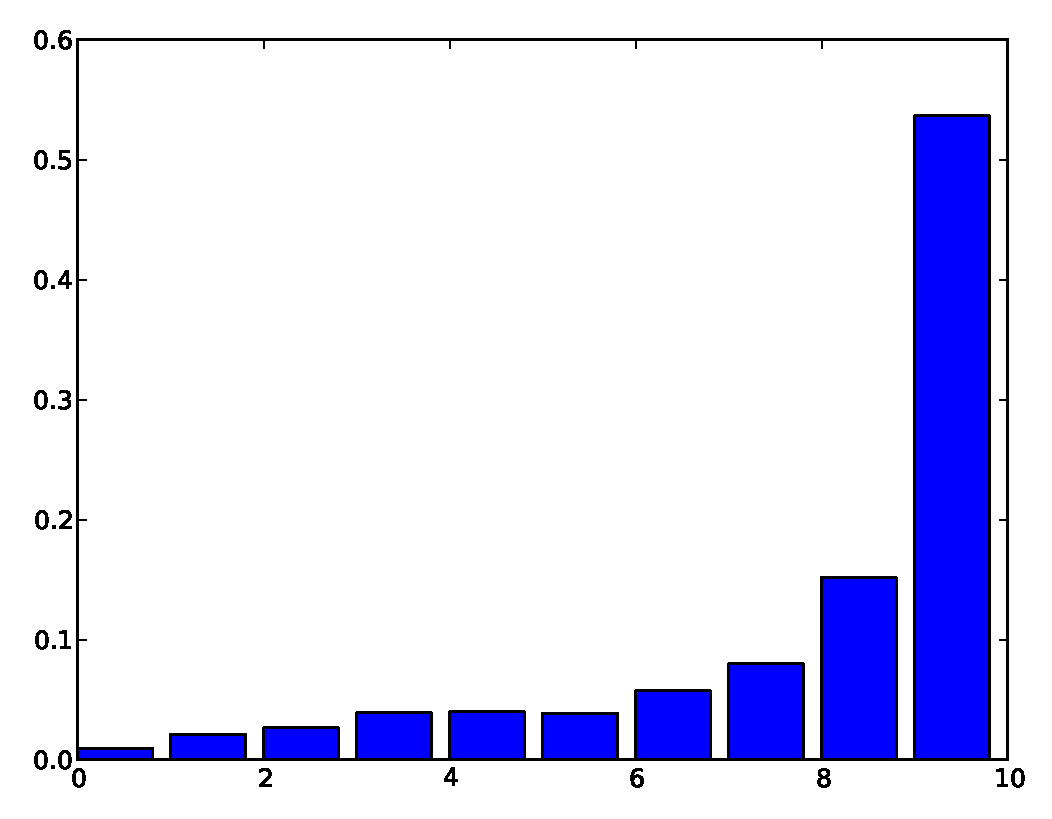
\includegraphics[width=\textwidth]{images/hist3}
                \caption{Diskretizovaný gausián}
                \label{fig:clf-discretisation-3}
        \end{subfigure}
        \caption[Diskretizácia výstupu klasifikátora]{Dve možnosti diskretizácie výstupu klasifikátora: buď použijeme histogram \ref{fig:clf-discretisation-1}, alebo dáta najskôr aproximujeme pomocou zmesi gausiánov \ref{fig:clf-discretisation-2} a následne zdiskretizujeme ako na obr. \ref{fig:clf-discretisation-3}.}
        \label{fig:clf-discretisation}
\end{figure}

\begin{table}[h]
\catcode`\-=12
\centering
\begin{tabular}{lrc}
\toprule
& počet košov & Úspešnosť\\
\midrule
Histogram & 10 & 81,78\%\\
 & 20 & 81,35\%\\
 & 50 & 59,97\%\\
Diskretizovaný gausián & 10 & 81,80\%\\
 & 20 & 81,55\%\\
 & 50 & 81,20\%\\
 & 100 & 81,12\%\\
Spojitý model & --- & 65,59\%\\
\bottomrule
\end{tabular}
\vspace{0.5cm}
\caption[Porovnanie úspešností pri rôznom spracovaní pásky]{Porovnanie úspešností modelu B pri rôznom spracovaní pásky a rôznom počte košov pri diskretizacii.}
\label{tab:success-b-tape}
\end{table}

Ako vidíme z~tabuľky \ref{tab:success-b-tape}, spojitá verzia modelu sa nám neosvedčila. Má totiž nedostatok, že distribučná funkcia nedosahuje maximum pri výstupe klasifikátora rovnom jedna, ale kúsok predtým, čo znamená istú penalizáciu v~prípade, že si je klasifikátor príliš istý.
Môžme si tiež všimnúť prudký pokles úspešnosti pri diskretizácii pomocou histokgramu s počtom košov 50. Je to spôsobené tým, že na trénovacej množine klasifikátor nevrátil žiadne hodnoty pre niektoré koše. Preto je rozumné použiť vyhladenie pomocou gausiánu, kde sa takéto problémy vyriešia. Okem toho bola úspešnosť s použitím gausiánu trochu vyššia ako bez neho takmer na všetkých testovaných sekvenciách.

\section{Trénovanie modelov}
\label{sec:model-training}

Na testovanie úspešnosti klasifikátora sme použili tri typy množín, ktoré si označíme \textit{simulované 1 (skr. sim1)}, \textit{simulované 2 (sim2)} a \textit{biologické (bio)}

Každá dátová množina sa skladá z troch podmnožín -- množina na trénovanie klasifikátora, množina na trénovanie modelu a testovacia množina.
Množina na trénovanie modelu totiž musí byť nezávislá od množiny na trénovanie modelu, pretože model budeme tiež používať na nezávisej množine a ak by sme použili tú istú množinu aj na trénovanie klasifkátora aj modleu, tak by model bol vychylený.

Množiny pre simulované dáta pozostávajú z 20 zarovnaní s dĺžkou 10000 pre trénovanie klasifikátora, jedného zarovnania s dĺžkou 10000 pre trénovanie modelu a 6 zarovnaní s dĺžkou 1000 pre testovanie modelu.
Množina biologických dát pre trénovanie klasifikátora sa skladala z 30 sekvencií s dĺžkami od 1000 do 1500, trénovacia množina pre modely obsahuje 41 sekvencií s dĺžkou od 1000 do 2500 a testovacia množina sa skladá zo 6 sekvencií s dĺžkami od 1000 do 1500.

V simulovaných dátach sme použili jednu anotáciu, ktorá označovala, či ide o gén, alebo nie.
Simulované dáta 1 boli vygenerované našim simulátorom, ktorý je popísaný v kapitole \ref{subsec:simulator}.
Simulované dáta 2 boli vygenerované tiež našim simulátorom, ktorý bol upravený tak, že v prípade génov sa sekvencie generovali z dvoch komplementárnych sekvencií a mimo génov z rovnakých sekvencií. Napríklad v prípade genov by sa namiesto AA vygenerovalo AT. To malo za úlohu posilniť význam anotácie.
Biologické dáta boli prevzaté z databázy génov UCSC (\cite{karolchik2003ucsc}) a išlo o multi zarovnanie 7 sekvencií.
Z nich sme si vybrali tri organizmy: človek (hg19), šimpanz(Pan troglodytes, panTro2) a pes (Canis familiaris, canFam2).
Ako anotácie sme použili dáta z programu genscan\footnote{program na hľadanie génov} a anotáciu s opakovaniami. Obe anotácie sme mali tiež z databázy génov UCSC.

% \begin{table}
% \centering
% \begin{tabular}{cccc}
% \toprule
% anotácia $X$ & anotácia $Y$ & sim1 & sim2\\
% \midrule
% 1 & 1 & 0,20 & 0,01\\
% 1 & 0 & \multirow{2}{*}{0,35} & \multirow{2}{*}{0,30}\\
% 0 & 1\\
% 0 & 0 & 0,40 & 0,99\\
% \bottomrule
% \end{tabular}
% \caption[Pravdepodobnosť mutácie v~našich datasetoch]{Pravdepodobnosť mutácie v~simulovaných dátach 1 a 2}
% \label{tab:sim-params}
% \end{table}

Naše modely trénujeme pomocou metódy maximálnej vierohodnosti, tak ako sme si to popísali v~kapitole \ref{subsec:hmmtraining}. V HMM trénujeme prechodové a emisné pravdepodobnosti. Prechodové pravdepodobnosti sme trénovali vo všetkých modeloch rovnako a emisné pravdepoodbnosti rôzne.

V~modeli~A~sme trénovali iba prechodové pravdepodobnosti, emisie sme mali priamo z~natrénovaného klasifikátora.

V~modeli~B sme trénovali aj prechodové aj emisné pravdepodobnosti.
Označme si bázy v sekvenciách $X, Y$ a výstup klasifikátora $C$. Veľkými písmenami $X, Y, C$ budeme označovať náhodné premenné pre bázy a výstup klasifikátora, malými písmenami budeme označovať konkrétne hodnoty. V match stave generujeme trojice: $(x, y, c)$ a v Inzert stavoch generujeme dvojice $(x, c)$ alebo $(y, c)$. Popíšeme si len trénovanie emisií v Match stave, Inzert stavy trénujeme analogicky. V diskrétnej verzii modelu si potrebujeme, vyrobiť tabuľku $e[x, y, c] = P(X=x, Y=y, C=c)\quad \forall x, y, c$. V spojitej verzii si potrebujeme zapamätať hustotu $C$ pre každú možnú dvojicu $(x, y)$. Teda budeme mať tabuľku $e[x, y] = f_{x,y}(t)\quad \forall x, y$, kde $f_{x,y}(t)$ je hustota náhodnej premennej $C$ za predpokladu, že $X=x$ a $Y=y$.
Keďže distribúciu $C$ chceme počítať pre každú možnú dvojicu báz zvlášť, musíme si ukázať, že pravdepodobnosť $P(X=x, Y=y, C=c)$ vieme rozložiť pomocou $P(C|X \cap Y)$. To vyplýva priamo z definície podmienenej pravdepodobnosti:
$$P\left(C=c \wedge X=x \wedge Y=y\right) = P\left(C=c | X=x \wedge Y=y\right) P\left(X=x \wedge Y=y\right)$$
%  Pri trénovaní emisií sme však urobili malú zmenu. Aby sme vedeli ľahko interpolovať vstupnú vzorku a~z~dôvodu lepšej vizualizácie sa nám hodí modelovať pravdepodobnosti $P(C|X \cap Y)$ (resp. $P(C|X)$ a $P(C|Y)$). Ukážeme si, že pravdepodobnosť $P(X \cap Y \cap C)$ vieme rozložiť pomocou $P(C|X \cap Y)$ a $P(X \cap C)$ vieme rozložiť pomocou $P(C|X)$.

% $P(X \cap Y)$ poznáme z~frekvenčnej tabuľky a $P(C)$ vieme rozložiť pomocou nasledujúcej vety.

% \begin{vt}[Veta o~úplnej pravdepodobnosti]
% Nech $A_1\dots A_n$ tvoria rozklad univerza~$\Omega$ a nech $B$ je udalosť, potom
% $$P(B) = \sum_{i=1}^n P(B|A_i)P(A_i)$$
% \end{vt}

% Máme teda
% $$P\left[C=c\right] = \sum_{\forall x\in X, y \in Y} P\left[C=c | X=x \wedge Y=y\right] P\left[X=x \wedge Y=y\right],$$
% pričom druhý člen poznáme a $P\left[C=c | X=x \wedge Y=y\right]$ už vieme ľahko dopočítať. Keď máme fixnuté dve bázy, vieme vybrať z~trénovacej sekvencie všetky pozície, kde sú zarovnané tieto bázy a vypočítať distribúciu C.

% Pre Indel stav postupujeme analogicky, ibaže namiesto $P(X \cap Y)$ máme buď $P(X)$ alebo $P(Y)$ podľa toho, ktorý stav práve počítame.

% Vieme teda pravdepodobnosť emisie $(x, y, c)$ Match stave vypočítať ako $$P\left[C=c \wedge X=x \wedge Y=y\right] = P\left[C=c | X=x \wedge Y=y\right] P\left[X=x \wedge Y=y\right]$$ a pravdepodobnosť emisie $(x, c)$ resp. $(y, c)$  v~Inzert stavoch pomocou
% \begin{align*}
% P\left[C=c \wedge X=x\right] &= P\left[C=c | X=x\right] P\left[X=x\right]\\
% P\left[C=c \wedge Y=y\right] &= P\left[C=c | Y=y\right] P\left[Y=y\right].
% \end{align*}
% Emisie môžme teda natrénovať zvlášť pre každú dvojicu báz (resp. pre každú bázu).

\section{Výsledky experimentov}
V~tejto sekcii sme porovnáme naše výsledky s~výsledkami referenčného modelu a zarovnávača \textit{muscle} \cite{edgar2004muscle} na našich troch dátových množinách popísaných v sekcii~\ref{sec:model-training}.

Potom uvedieme výsledky nikoľkých experimentov, v ktorých sme porovnávali naše modely s rôznymi parametrami a v rôznych podmienkach.

Keďže k biologickým dátam nepoznáme správne zarovnanie, rozhodli sme sa zaviesť okrem percentuálnej zhody ďalšiu mieru. Túto mieru budeme označovať \textit{tranzitivita} a budeme ju počítať z troch párových zarovnaní, ktoré dostaneme z troch sekvencií zarovnaním všetkých ich kombinácií. Označme si tri  sekvencie ako $A, B, C$. Vyrobíme si tri zarovnania: $AB, BC$ a $AC$. Tranzitivitu spočítame ako percentuálnu zhodu medzi zložením prvých dvoch zarovnaní ($AB \circ BC$) a tretieho zarovnania $AC$. V ideálnom prípade by sme dostali 100\% a mali by sme multizarovnanie troch sekvencií. V praxi sú však hodnoty nižšie.
Táto miera určuje konzistentnosť zarovnávača, čo je jedna z dôležitých vlastností kvalitného zarovnávača. V prípade biologických dát považujeme túto mieru za dôležitejšiu, pretože v tomto prípade náš zarovnávač môže nájsť biologicky správnejšie zarovnanie ako bolo to pôvodné. Avšak my sme si na naše testy vybrali multizarovnania 7 sekvencií, ktoré sú považvané za veľmi kvalitné. Preto budeme požadovať aj vysoké percento zhody ako sekundárne kritérium.

\begin{table}[htp]
\catcode`\-=12
\centering
\begin{tabu} to \textwidth {X[l]X[c]X[c]X[c]X[c]X[c]X[c]X[c]X[c]}
\toprule
\multirow{2}{*}{Dáta} &
\multicolumn{2}{c}{Model A} &
\multicolumn{2}{c}{Model B } &
\multicolumn{2}{c}{Ref. Model } &
\multicolumn{2}{c}{Muscle} \\
\cmidrule(r){2-3}\cmidrule(lr){4-5}\cmidrule(lr){6-7}\cmidrule(l){8-9}
& Zhoda & Tranz. & Zhoda & Tranz. & Zhoda & Tranz. & Zhoda & Tranz.\\
\midrule
sim1 & 79,75\% & 44,97\% & 84,35\% & 56,5\% & \textbf{85,78\%} & \textbf{61,03\%} & 82,72\%& 58,76\%\\
sim2 & 70,14\% & --- & \textbf{71,47}\% & --- & 60,38\% & --- & 61,47\% & --- \\
bio & \textbf{91,40\%} & 96,63\% & 91,24\% & \textbf{96,89\%} & 91,34\% & 96,45\% & 91,28\% & 95,98\%\\
\bottomrule
\end{tabu}
\caption[Porovnanie s~existujúcimi zarovnávačmi]{Porovnanie našich modelov s~referenčným modelom a zarovnávačom muscle.}
\label{tab:success-compare}
\end{table}

V~tabuľke \ref{tab:success-compare} sme porovnávali naše modely so základným modelom a zarovnávačom muscle. Typ dát v našich expeimentoch je typ D a okno je veľkosti 9.
Na simulovaných dátach, ktoré boli generované náhodne, naše modely nedokázali prekonať referenčné modely.
Keď sme však posilnili význam anotácie (simulované dáta 2) referenčné modely, ktoré anotáciu k dispozícii nemali boli v nevýhode a naše modeli dopadli lepšie.
Na biologických dátach, v ktorých je viacej pravidelností ako v simulovaných, dokázali dodatočné informácie pomôcť dosiahnuť lepšiu tranzitivitu (čo bol v tomto prípade náš primárny cieľ) a v prípade modelu A aj lepšiu úspešnošť.

Naše modely produkujú porovnateľné výsledky, avšak model B bol vo väčšine prípadov lepší. Model B je totiž kombináciou pôvodného pHMM a modelu A. Na rozdiel od modelu A sa nespolieha len na výsledky klasifikácie, pri korých sa občas môže stať, že niesú dobré (úspešnosť je len okolo 80\%), ale aj na samotné frekvencie výskytov dvojíc písmen. Klasifikátor potom na základe dodatočnej informácie upravuje túto pravdepodobnosť.

% Model A~emituje len na základe natrénovaného klasifikátora, takže čokoľvek dokážeme klasifikátor naučiť, môžme priamo použiť. Model B používa klasifikátor iba ako pomôcku, funguje podobne ako štandardný model pre zarovnanie (sekcia \ref{subsec:hmm-alignment}) a klasifikátor iba mierne upravuje výsledné pravdepodobnosti. Model B je teda viazaný aj pravdepodobnosťami výskytov dvojíc báz.


% ako sa modely dokážu prispôsobiť zložitejším dátam. Môžme si všimnúť, že model A~sa správa konzistentne na oboch typoch dát, zatiaľ čo model B sa pri zložitejšom type dát nechal stiahnuť dole nutnosťou dodržovať pravdepodobnosti generovania báz.


% \begin{table}
% \centering
% \begin{tabular}{ccc}
% \toprule
% bázy & výstup klasifikátora & emis. pravd.\\
% \midrule
% AA & 0.96 & 0,09399\\
% AG & 0.96 & 0,00513\\
% AA & 0.42 & 0,00729\\
% AA & 0.26 & 0,00411\\
% AG & 0.02 & 0,00168\\
% \bottomrule
% \end{tabular}
% \caption[Porovnanie emisných pravdepodobností]{Porovnanie emisných pravdepodobností pre rôzne bázy a výstup natrénovaného klasifikátora}
% \label{tab:emission-prob}
% \end{table}

% Ako môžme v~tabuľke \ref{tab:emission-prob} vidieť, pre rovnaký výstup klasifikátora, ale rôzne bázy sa emisná pravdepodobnosť môže líšiť. Dokonca aj pre značne nižší výstup klasifikátora pri rovnakých bázach môže byť pravdepodobnosť emisie stále vyššia ako pri rôznych bázach s~vysokým výstupom z~klasifikátora. Na druhej strane si môžme tiež všimnúť, že pri nižšom výstupe klasifikátora emisná pravdepodobnosť rapídne klesá a pri dostatočne nízkom výstupe klasifikátora pri rovnakých bázach už je emisná pravdepodobnosť nižšia, ako pri rôznych bázach s~vysokým výstupom klasifikátora.

% \begin{table}[htp]
% \todo pregenerovať s~oknom 9\\
% \centering
% \begin{tabular}{crrr}
% \toprule
% & Model A~& Model B & Ref. model\\
% \midrule
% Simulované 1 & 79,75\% & 84,35\% & 85,78\%\\
% Simulované 2 & 72,62\% & 18,57\% & 6,78\% \\
% \bottomrule
% \end{tabular}

% \caption[Porovnanie úspešností modelov]{Porovnanie úspešností modelov. Referenčný model je obyčajný pHMM na zarovnávanie DNA sekvencií. Úspešnosť je počítaná ako percentuálna zhoda originálneho a nového zarovnania. Simulované dáta 1 sa snažia napodobňovať biologické procesy, Simulované dáta 2 nezodpovedajú biologickým dátam a sú zložitejšie na natrénovanie pre referenčný model.}
% \label{tab:success-compare}
% \end{table}

% \subsection{Rôzne veľkosti okna}

% V~tejto sekcii sme sa venovali hľadaniu optimálnej veľkosti okna. Vyskúšali sme viacero možností a výsledky sme zapísali do tabuľke \ref{tab:window-compare}.

% \begin{table}[htp]
% \centering
% \begin{tabular}{ccc}
% \toprule
% Veľkosť okna & Model A~& Model B\\
% \midrule
% 1 & 76,95\% & 57,86\%\\
% 3 & 70,62\% & 81,42\%\\
% 5 & 73,95\% & 82,98\%\\
% 7 & 78,31\% & 83,05\%\\
% 9 & 79,75\% & 84,35\%\\
% 11 & 79,28\% & 83,57\%\\
% 13 & 80,58\% & 83,98\%\\
% 15 & 81,62\% & 83,98\%\\
% \bottomrule
% \end{tabular}
% \caption[Porovnanie úspešností pri rôznej veľkosti okna]{Porovnanie úspešností modelov pri rôznej veľkosti okna.}
% \label{tab:window-compare}
% \end{table}

% Z~tabuľky vidíme, že pre model B je optimálna veľkosť okna 7-9, pri väčších oknách už úspešnosť nerastie. Pri modeli A~rástla úspešnosť až po veľkosť okna 15. Optimálnu hodnotu pre model A~sme na základe tabuľky určili na 9-15.

\subsection{Vplyv dodatočnej informácie na zarovnanie}

V~tejto sekcii sme zisťovali, aký vplyv má dodatočná informácia na zarovnanie v simulovaných dátach 1. Porovnali sme štyri scenáre:
\begin{itemize}
    \item okno veľkosti jedna bez anotácie -- zodpovedá tomu, čo vidí aj základný pHMM
    \item okno veľkosti jedna s anotáciou -- obsahuje navyše iba anotáciu
    \item okno veľkosti 9 bez anotácie -- obsahuje navyše iba okolie v sekvencii
    \item okno veľkosti 9 s anotáciou -- obsahuje navyše okolie v sekvencii aj anotácii
\end{itemize}

\begin{table}[htp]
\centering
\begin{tabular}{cccc}
\toprule
Veľkosť okna & Anotácia & Model A~& Model B\\
\midrule
1 & nie & 74,42\% & 18,35\%\\
1 & áno & 76,95\% & 57,86\%\\
\noalign{\vskip 2mm}
9 & nie & 78,43\% & 82,67\%\\
9 & áno & 79,75\% & 84,35\%\\
\bottomrule
\end{tabular}
\caption[Vplyv dodatočnej informácie na zarovnanie]{Vplyv dodatočnej informácie na zarovnanie.}
\label{tab:annotation-compare}
\end{table}

V~tabuľke \ref{tab:annotation-compare} si môžeme všimnúť, že zatiaľ čo pri modeli A~je úspešnosť veľmi podobná, hoci aj anotácie aj väčšie okno mierne pomohli. Naopak pri modeli B sú rozdiely výrazne väčšie, vidíme, že aj samotná anotácia výrazne pomohla a väčšie okno je pre tento model nutnosťou. Pri menšom počte atribútov totiž klasifikátor môže vrátiť len malý počet rôznych hodnôt (maximálne toľko, koľko je možných vstupov), čo je v modeli B nedostatočné. V modeli A to až tak nevadí, pretože v tomto prípade sa bude správať podobne ako pHMM -- pre rovnaké bázy bude dávať vyššie hodnoty a pre rôzne nižšie.

\subsection{Použitie jedného klasifikátora pre Match aj Inzert stav}
V tejto sekcii si ukážeme, že voľba dvoch špecializovaných klasifikátorov mala svoje opodstatnenie. Namiesto dvoch špecifických klasifikátorov sme použili jeden klasifikátor aj pre Match aj pre Inzert stav. Tento klasifikátor bol taký istý ako náš Match klasifikátor a v Inzert stave sme prevrátili jeho hodnotu. Tieto možnosti sme porovnali na simulovaných dátach 1.

\begin{table}[htp]
\centering
\begin{tabular}{lcc}
\toprule
 & Model A~& Model B\\
\midrule
1 klasifikátor & 74,53\% & 82,72\%\\
2 klasifikátory & 79,75\% & 84,35\%\\
\bottomrule
\end{tabular}
\caption[Porovnanie použitia jedného alebo dvoch typov klasifikátorov]{Porovnanie použitia jedného alebo dvoch typov klasifikátorov.}
\label{tab:1clf-compare}
\end{table}

Z~tabuľky \ref{tab:1clf-compare} vidíme, že hoci naše modeli dokážu fungovať aj s jedným klasifikátorom, použitie dvoch typov klasifikátorov má svoje opodstatnenie a zvyšuje úspešnosť klasifikatorov.

\section{Zhrnutie}

V tejto kapitole sme si predstavili dva modely pre zarovnávanie sekvencií s dodatočnou informáciou pomocou klasifikátorov: model A a model B.
Oba modely boli založené na pHMM. Prvý z nich priamo nahradil emisné pravdepodobnosti výstupom klasifikátora, a teda nemôže byť považovany za pravdepodobnostný model.
Druhý model sme navrhli ako pravdepodobnostný model, a okrem dvoch sekvencií mal k dispozícii pásku s výstupom z klasifikátorov. Uviedli sme si aj spôsob diskretizácie výstupu klasifikatora pre model B.

Ukázali sme, že na biologických dátach dokážu naše modely prekonať úspešnosť referenčných modelov. Okrem toho sme ukázali, že naše modely sú na rozdiel od referenčných modelov použiteľné aj v prípade, že vlastnosti zarovnania veľmi závisia od anotácie.

Nakoniec sme si ukázali aj opodstatnenie dvoch typov klasifikátorov namiesto jedného a aj to, že anotácia aj väčšie okolie daných báz majú pozitívny vplyv na zarovnávanie našimi modelmi.
